\chapter{Design and Implementation}\label{chp:designimpl}
This chapter suggests a prototype implementation of one possible application, on background of the principles and ideas in the previous two sections. The protocol structure will be displayed, together with examples from the code and test runs using the system.

\section{System specifications}\label{sec:chat}
As mentioned in \ref{sec:apps} there are several scenarios where functional key exchange can provide security and privacy. This section will describe the structure and specifications for a chat system utilizing \gls{abake} as described in \ref{sec:abake} and \cite{DBLP:abake}. The system consists of a set of clients running a client application and a broadcast server. It could easily have been altered to support peer-to-peer, since the server only acts as a intermediate for broadcasting, caching of encapsulations and policy management. The system shown is meant to be a proof of concept for how this kind of application could look, it is thus simplified to some extent. Most of the data used are static to abstract away difficulties with administration of rooms and related policies, as well as key management. The implementation will not address key distribution, therefor a key is given to the users on connection. The extended system would include a separate \gls{kms} which the users would register with to obtain their key. The best solution would probably be to have a separate virtual or physical server doing each task; attribute and key management, storage and distribution of keying material, broadcasting of chat messages/cipher texts. Other features like being able to create your own rooms and administrate these would also be logical. This prototype will be a single room with a static policy.
\paragraph{The most important feature} of the system is to provide encrypted communication between users whom satisfy the room policy. The users should obtain a shared session key through \gls{abake}. This way we assure implicit authentication of all users taking part in the conversation. A user should be able to participate in the exchange without ever having to provide an identity. It is assumed that all users have registered with some \gls{kms} prior to the key exchange, a user would typically register a set of attributes which would have to be approved by the system authority. When new users join, they should be able to upload their contribution and receive the rest of the keying material from the server; the users will then have to compute the new session key. After exchanging keys, the users should be able to use it to encrypt the chat messages. It should be noted that anybody can in fact upload a contribution and receive encapsulations, but only the ones with the correct attributes can decapsulate and produce the session key. It might be smart for the server to challenge the new user to prove that he has the correct attributes.


\section{Models and construction}
The high level construction of the key exchange used in the system is based on the generic one-round AB-AKE protocol presented by Gorantal et al. \cite{gorantla2010attribute}. The main differences being the encapsulation function used, the implementation described in this project is constructed based on the \gls{abe} scheme implemented in Charm, as described in \ref{subsec:ABE} and \cite{abe_waters09}, while \cite{gorantla2010attribute} introduce \gls{epabkem}. This project propose a complete system utilizing the key exchange, so after obtaining a shared key, users encrypt their messages using a standard symmetric key encryption algorithm. The messages are broadcast through the same broadcast server used for key exchange. When a new user joins, the message exchanges are paused until the new key is calculated by all users. Figure \ref{fig:flow} shows the system flow when a new user connects. A client will first query the server for the room policy, before a encapsulation is generated from the received policy. This one is sent to the server which distributes it so that all users have all contributions. After doing this distribution, the server will go back to being a pure broadcast server for chat messages. Figure \ref{fig:encapdistr} illustrates the encapsulation distribution process. Bob is a new user, so he uploads his contribution to the server, there are $n$ users already in the system. Next the server broadcast Bob's encapsulation to the current users, before sending the set of active encapsulations to Bob.



\begin{figure}
\centering
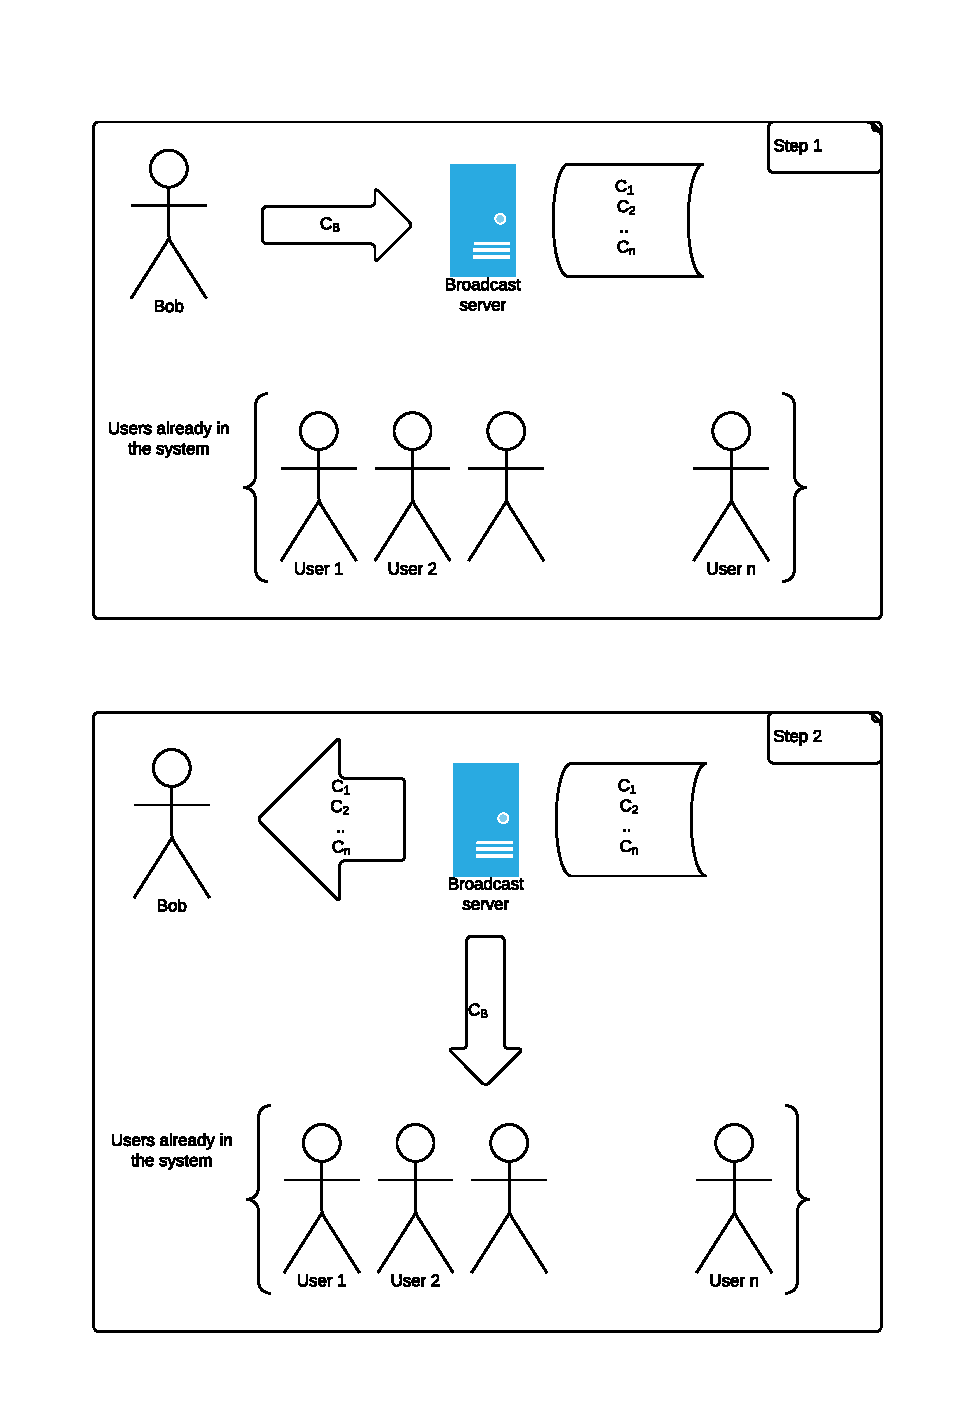
\includegraphics[trim=2cm 1.5cm 2cm 4cm ,scale=1]{chatsystem.pdf}
\caption{Distribution of encapsulations}
\label{fig:encapdistr}
\end{figure}

\begin{figure}
\centering
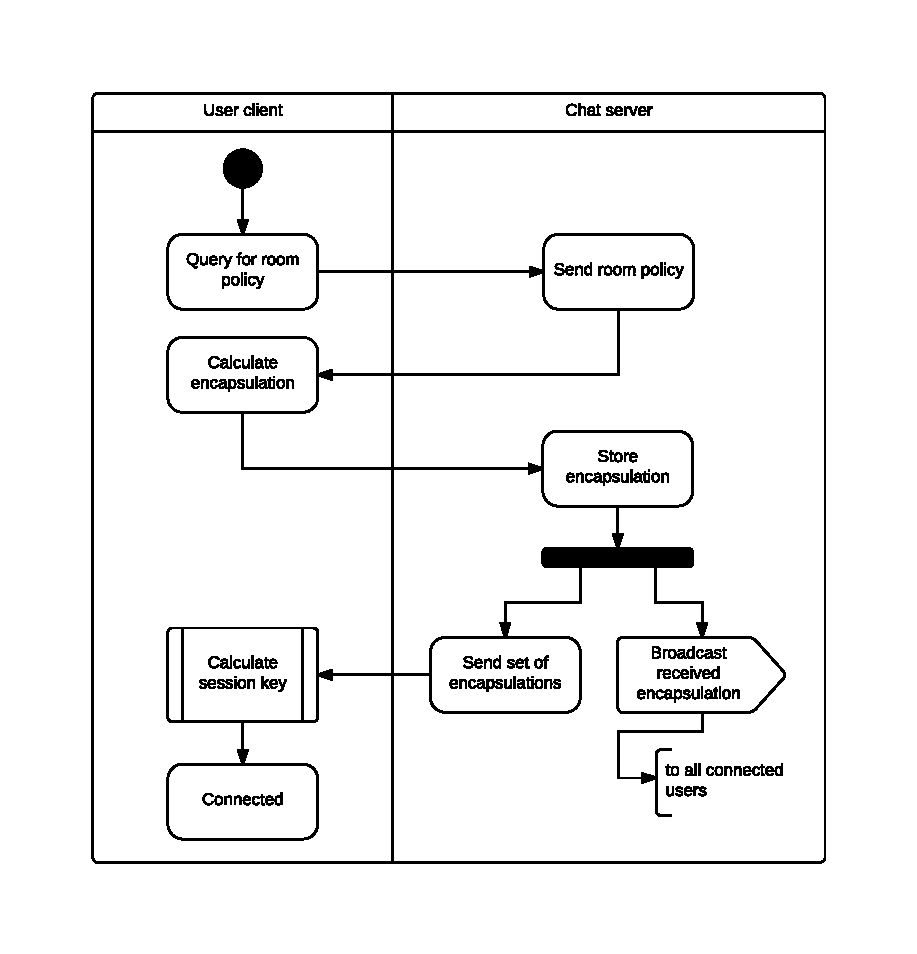
\includegraphics[trim=2cm 2cm 0cm 1cm ,scale=1]{Flow.pdf}
\caption{System flow.}
\label{fig:flow}
\end{figure}




\section{Implementation}
The application will consist of to components, one server class and one client class. The implementations of these follow the state diagrams \ref{fig:server-state} and \ref{fig:client-state} respectively. This section will describe how these two classes are implemented, the complete implementation including the code is attached in 
\subsection{Server program} 

\begin{figure}
\centering
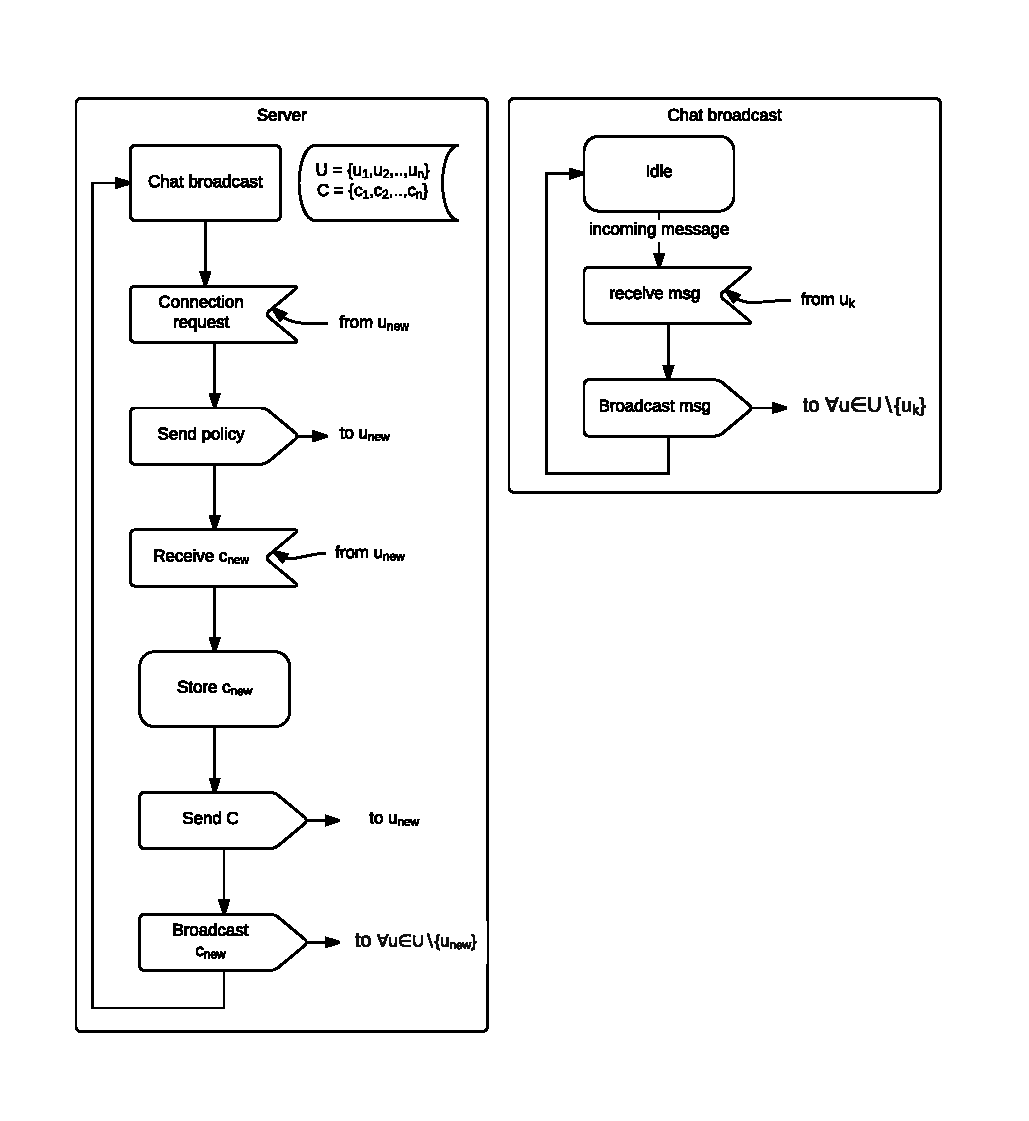
\includegraphics[trim=2cm 1.5cm 2cm 4cm ,scale=1]{server-state.pdf}
\caption{Internal flow of the server class}
\label{fig:server-state}
\end{figure}


\subsection{Client program}


\begin{figure}
\centering
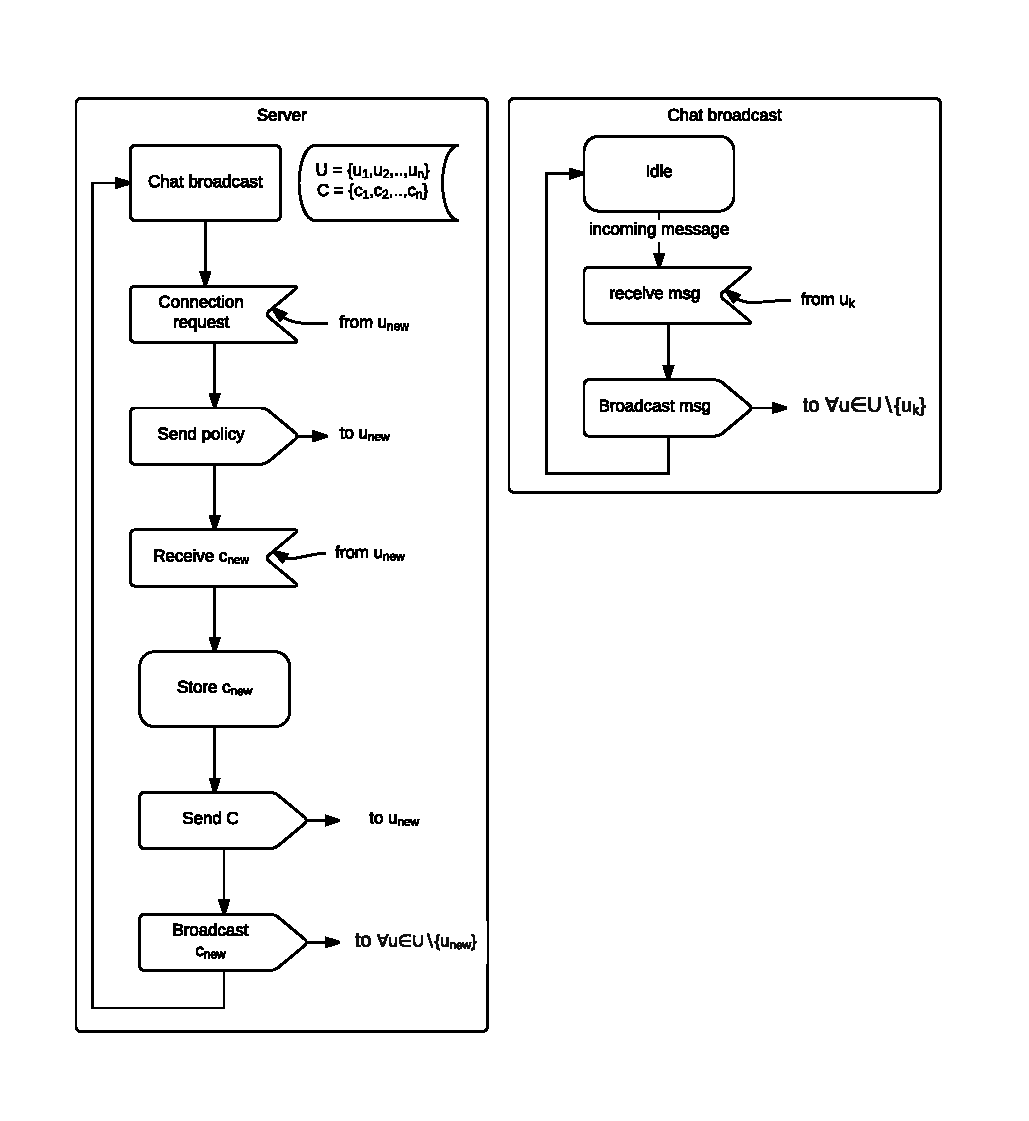
\includegraphics[trim=2cm 1.5cm 2cm 4cm ,scale=1]{server-state.pdf}
\caption{Internal flow of the client class}
\label{fig:client-state}
\end{figure}

\section{System demonstration}


